\documentclass[../../InformazioneQuantistica.tex]{subfiles}

\begin{document}

\section{Teletrasporto quantistico}
\lesson{3 \greendot}{6/3/2019}
L'idea del teletrasporto quantistico\index{Teletrasporto quantistico} consiste nel partire da un \textbf{qubit}, definito da una funzione d'onda generica $\ket{\psi}$ \textbf{non nota}, e trasmettere l'informazione in esso contenuta ad un qubit di un altro laboratorio. Dato che non è possibile \textbf{clonare} $\ket{\psi}$, il teletrasporto ha come effetto la distruzione del qubit originale.\\
\textbf{Nota}: stiamo comunque parlando di un trasporto di \textbf{informazione}, non di materia. Nel laboratorio di arrivo deve essere presente una particella a cui \q{applicare} il qubit trasportato.\\

Il protocollo di teletrasporto quantistico che esamineremo richiede:
\begin{itemize}
\item Due qubit in uno stato EPR (cioè in stato \textit{massimamente entangled}), che vengono separati e portati uno al laboratorio di Alice ($A$) e l'altro a quello di Bob ($B$).
\item Un qubit (C) nel laboratorio di Alice il cui contenuto sarà \textit{teletrasportato} nel qubit $B$ di Bob.
\item Due bit classici che permettano ad Alice di registrare il risultato di due misurazioni, e trasmettere tale esito a Bob mediante un \textit{canale di comunicazione classico}. Poiché tale passaggio di informazione può avvenire solo a velocità $v < c$, si ha che il teletrasporto quantistico non può essere un processo superluminale, e quindi non viola la relatività speciale. 
\end{itemize}

Consideriamo quindi il setup di figura \ref{fig:setup-sperimentale}.

\begin{figure}[H]
\centering


\tikzset{every picture/.style={line width=0.75pt}} %set default line width to 0.75pt        
\begin{center}
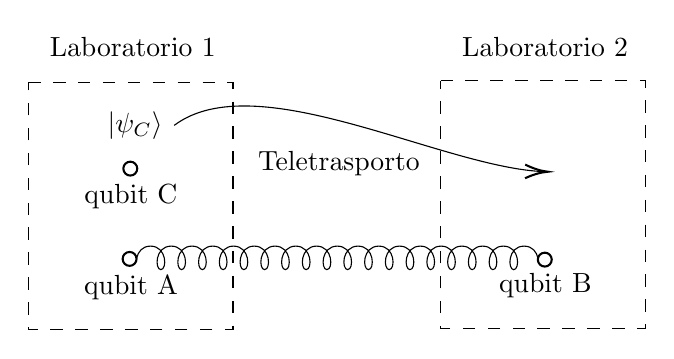
\begin{tikzpicture}[x=0.75pt,y=0.75pt,yscale=-1,xscale=1]
%uncomment if require: \path (0,300); %set diagram left start at 0, and has height of 300

%Shape: Rectangle [id:dp019828091081898647] 
\draw  [dash pattern={on 4.5pt off 4.5pt}] (101,91.17) -- (199.67,91.17) -- (199.67,210.5) -- (101,210.5) -- cycle ;
%Shape: Rectangle [id:dp7316415823282396] 
\draw  [dash pattern={on 4.5pt off 4.5pt}] (299.67,90.5) -- (398.33,90.5) -- (398.33,209.83) -- (299.67,209.83) -- cycle ;
%Shape: Spring [id:dp4458037239709285] 
\draw   (153.29,175.83) .. controls (153.92,173) and (155.92,170.17) .. (159.92,170.17) .. controls (167.92,170.17) and (167.92,181.5) .. (164.92,181.5) .. controls (161.92,181.5) and (161.92,170.17) .. (169.92,170.17) .. controls (177.92,170.17) and (177.92,181.5) .. (174.92,181.5) .. controls (171.92,181.5) and (171.92,170.17) .. (179.92,170.17) .. controls (187.92,170.17) and (187.92,181.5) .. (184.92,181.5) .. controls (181.92,181.5) and (181.92,170.17) .. (189.92,170.17) .. controls (197.92,170.17) and (197.92,181.5) .. (194.92,181.5) .. controls (191.92,181.5) and (191.92,170.17) .. (199.92,170.17) .. controls (207.92,170.17) and (207.92,181.5) .. (204.92,181.5) .. controls (201.92,181.5) and (201.92,170.17) .. (209.92,170.17) .. controls (217.92,170.17) and (217.92,181.5) .. (214.92,181.5) .. controls (211.92,181.5) and (211.92,170.17) .. (219.92,170.17) .. controls (227.92,170.17) and (227.92,181.5) .. (224.92,181.5) .. controls (221.92,181.5) and (221.92,170.17) .. (229.92,170.17) .. controls (237.92,170.17) and (237.92,181.5) .. (234.92,181.5) .. controls (231.92,181.5) and (231.92,170.17) .. (239.92,170.17) .. controls (247.92,170.17) and (247.92,181.5) .. (244.92,181.5) .. controls (241.92,181.5) and (241.92,170.17) .. (249.92,170.17) .. controls (257.92,170.17) and (257.92,181.5) .. (254.92,181.5) .. controls (251.92,181.5) and (251.92,170.17) .. (259.92,170.17) .. controls (267.92,170.17) and (267.92,181.5) .. (264.92,181.5) .. controls (261.92,181.5) and (261.92,170.17) .. (269.92,170.17) .. controls (277.92,170.17) and (277.92,181.5) .. (274.92,181.5) .. controls (271.92,181.5) and (271.92,170.17) .. (279.92,170.17) .. controls (287.92,170.17) and (287.92,181.5) .. (284.92,181.5) .. controls (281.92,181.5) and (281.92,170.17) .. (289.92,170.17) .. controls (297.92,170.17) and (297.92,181.5) .. (294.92,181.5) .. controls (291.92,181.5) and (291.92,170.17) .. (299.92,170.17) .. controls (307.92,170.17) and (307.92,181.5) .. (304.92,181.5) .. controls (301.92,181.5) and (301.92,170.17) .. (309.92,170.17) .. controls (317.92,170.17) and (317.92,181.5) .. (314.92,181.5) .. controls (311.92,181.5) and (311.92,170.17) .. (319.92,170.17) .. controls (327.92,170.17) and (327.92,181.5) .. (324.92,181.5) .. controls (321.92,181.5) and (321.92,170.17) .. (329.92,170.17) .. controls (337.92,170.17) and (337.92,181.5) .. (334.92,181.5) .. controls (331.92,181.5) and (331.92,170.17) .. (339.92,170.17) .. controls (344,170.17) and (346,173.12) .. (346.58,176.01) ;
%Straight Lines [id:da8152639809390969] 
\draw    (149.83,176.33) ;

\draw [shift={(149.83,176.33)}, rotate = 0] [color={rgb, 255:red, 0; green, 0; blue, 0 }  ][line width=0.75]      (0, 0) circle [x radius= 3.35, y radius= 3.35]   ;
%Straight Lines [id:da6744702488611394] 
\draw    (150.17,132.83) ;

\draw [shift={(150.17,132.83)}, rotate = 0] [color={rgb, 255:red, 0; green, 0; blue, 0 }  ][line width=0.75]      (0, 0) circle [x radius= 3.35, y radius= 3.35]   ;
%Straight Lines [id:da8857801521218736] 
\draw    (349.87,176.67) ;

\draw [shift={(349.87,176.67)}, rotate = 0] [color={rgb, 255:red, 0; green, 0; blue, 0 }  ][line width=0.75]      (0, 0) circle [x radius= 3.35, y radius= 3.35]   ;
%Curve Lines [id:da07911679295346907] 
\draw    (171.33,112) .. controls (210.93,82.3) and (300.85,132.64) .. (349.86,134.3) ;
\draw [shift={(351.33,134.33)}, rotate = 180.78] [color={rgb, 255:red, 0; green, 0; blue, 0 }  ][line width=0.75]    (10.93,-3.29) .. controls (6.95,-1.4) and (3.31,-0.3) .. (0,0) .. controls (3.31,0.3) and (6.95,1.4) .. (10.93,3.29)   ;


% Text Node
\draw (151.33,74) node  [align=left] {Laboratorio 1};
% Text Node
\draw (350,74) node  [align=left] {Laboratorio 2};
% Text Node
\draw (150.5,190) node  [align=left] {qubit A};
% Text Node
\draw (150.5,146.5) node  [align=left] {qubit C};
% Text Node
\draw (152.5,112) node   {$|\psi _{C} \rangle $};
% Text Node
\draw (350.2,189) node  [align=left] {qubit B};
% Text Node
\draw (250.67,130.33) node  [align=left] {Teletrasporto};


\end{tikzpicture}
\end{center}
\caption{Setup sperimentale per il teletrasporto quantistico
\label{fig:setup-sperimentale}}
\end{figure}

Presso i laboratori di Alice e Bob sono disponibili i qubit $A$ e $B$, nello stato \textit{entangled} dato da:
\begin{align*}
\ket{\psi}_{AB} = \frac{1}{\sqrt{2}}(\ket{00}_{AB} +\ket{11}_{AB})
\end{align*}
Perciò se una misura di $A$ trova un risultato $0$ o $1$, una qualsiasi successiva misura di $B$ troverà lo stesso esito.\\

Alice ha poi anche il qubit $C$, nello stato generico $\ket{\psi_c}$ non noto, che vogliamo trasferire a Bob.\\

Mettendo tutto insieme, si ha che lo stato iniziale $\ket{\Phi}_{ABC}$ del sistema è dato da:
\begin{align*}
\ket{\Phi_0}_{ABC} = \ket{\psi}_C \otimes \left(\frac{\ket{00}+\ket{11}}{\sqrt{2}}\right)_{AB} \qquad \ket{\psi}_C = \alpha \ket{0}+\beta \ket{1}
\end{align*}

Il \textbf{protocollo} di teletrasporto quantistico consiste in una serie di operazioni che possiamo schematizzare come un \textbf{circuito quantistico} (figura \ref{fig:teletrasporto-circuito}).


\begin{figure}[H]
\centering


\tikzset{every picture/.style={line width=0.75pt}} %set default line width to 0.75pt        
\begin{center}
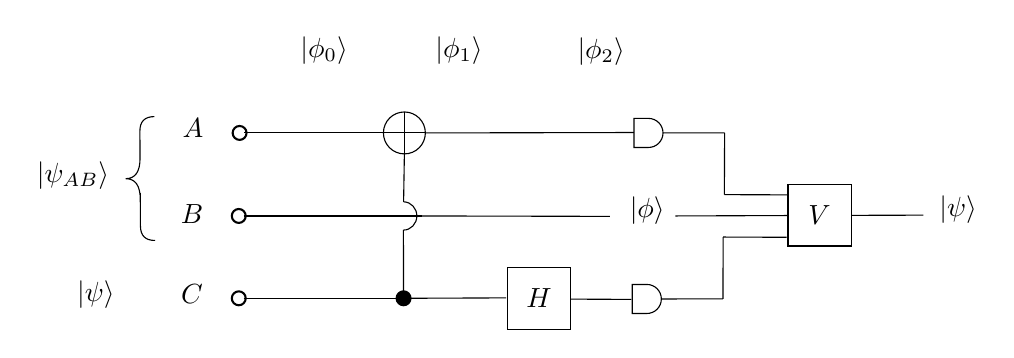
\begin{tikzpicture}[x=0.75pt,y=0.75pt,yscale=-1,xscale=1]
%uncomment if require: \path (0,300); %set diagram left start at 0, and has height of 300

%Straight Lines [id:da6069497950635481] 
\draw    (162.75,130.2) -- (239.8,130.2) ;

\draw [shift={(160.4,130.2)}, rotate = 0] [color={rgb, 255:red, 0; green, 0; blue, 0 }  ][line width=0.75]      (0, 0) circle [x radius= 3.35, y radius= 3.35]   ;
%Straight Lines [id:da9334857253899997] 
\draw    (162.35,170.2) -- (248.33,170.2) ;

\draw [shift={(160,170.2)}, rotate = 0] [color={rgb, 255:red, 0; green, 0; blue, 0 }  ][line width=0.75]      (0, 0) circle [x radius= 3.35, y radius= 3.35]   ;
%Straight Lines [id:da7800321309399463] 
\draw    (162.35,209.87) -- (239.4,209.87) ;
\draw [shift={(239.4,209.87)}, rotate = 0] [color={rgb, 255:red, 0; green, 0; blue, 0 }  ][fill={rgb, 255:red, 0; green, 0; blue, 0 }  ][line width=0.75]      (0, 0) circle [x radius= 3.35, y radius= 3.35]   ;
\draw [shift={(160,209.87)}, rotate = 0] [color={rgb, 255:red, 0; green, 0; blue, 0 }  ][line width=0.75]      (0, 0) circle [x radius= 3.35, y radius= 3.35]   ;
%Flowchart: Or [id:dp510436773552555] 
\draw   (229.7,130.2) .. controls (229.7,124.62) and (234.22,120.1) .. (239.8,120.1) .. controls (245.38,120.1) and (249.9,124.62) .. (249.9,130.2) .. controls (249.9,135.78) and (245.38,140.3) .. (239.8,140.3) .. controls (234.22,140.3) and (229.7,135.78) .. (229.7,130.2) -- cycle ; \draw   (229.7,130.2) -- (249.9,130.2) ; \draw   (239.8,120.1) -- (239.8,140.3) ;
%Shape: Arc [id:dp8694086567644008] 
\draw  [draw opacity=0] (239.42,163.4) .. controls (239.43,163.4) and (239.43,163.4) .. (239.44,163.4) .. controls (242.97,163.42) and (245.82,166.48) .. (245.8,170.24) .. controls (245.78,173.99) and (242.89,177.02) .. (239.36,177) .. controls (239.35,177) and (239.34,177) .. (239.33,177) -- (239.4,170.2) -- cycle ; \draw   (239.42,163.4) .. controls (239.43,163.4) and (239.43,163.4) .. (239.44,163.4) .. controls (242.97,163.42) and (245.82,166.48) .. (245.8,170.24) .. controls (245.78,173.99) and (242.89,177.02) .. (239.36,177) .. controls (239.35,177) and (239.34,177) .. (239.33,177) ;
%Straight Lines [id:da32732471404561303] 
\draw    (239.8,140.3) -- (239.42,163.4) ;


%Straight Lines [id:da9630089573088603] 
\draw    (239.33,177) -- (239.4,209.87) ;


%Straight Lines [id:da4509691261125206] 
\draw    (248.33,170.2) -- (338.8,170.4) ;


%Straight Lines [id:da22340016004613328] 
\draw    (239.4,209.87) -- (288.83,209.67) ;


%Shape: Rectangle [id:dp4916897596211902] 
\draw   (289.43,194.87) -- (319.85,194.87) -- (319.85,224.7) -- (289.43,224.7) -- cycle ;
%Straight Lines [id:da9818585232667203] 
\draw    (319.8,210.27) -- (349.2,210.4) ;


%Flowchart: Delay [id:dp03407065361349182] 
\draw   (349.6,203.2) -- (356.6,203.2) .. controls (360.47,203.2) and (363.6,206.33) .. (363.6,210.2) .. controls (363.6,214.07) and (360.47,217.2) .. (356.6,217.2) -- (349.6,217.2) -- cycle ;
%Straight Lines [id:da11659338543124176] 
\draw    (249.9,130.2) -- (350.4,130) ;


%Flowchart: Delay [id:dp8183178942903988] 
\draw   (350.4,123.2) -- (357.4,123.2) .. controls (361.27,123.2) and (364.4,126.33) .. (364.4,130.2) .. controls (364.4,134.07) and (361.27,137.2) .. (357.4,137.2) -- (350.4,137.2) -- cycle ;
%Shape: Rectangle [id:dp15653968669405383] 
\draw   (424.63,154.87) -- (455.05,154.87) -- (455.05,184.7) -- (424.63,184.7) -- cycle ;
%Straight Lines [id:da8427392636457767] 
\draw    (370.33,170.2) -- (424.4,170) ;


%Straight Lines [id:da7732960549801164] 
\draw    (364.4,130.2) -- (394.08,130.14) ;


%Straight Lines [id:da35329750543082605] 
\draw    (363.6,210.2) -- (393.28,210.14) ;


%Straight Lines [id:da8838324556439012] 
\draw    (393.28,210.14) -- (393.38,180.36) ;


%Straight Lines [id:da8616696291975874] 
\draw    (393.97,159.93) -- (394.08,130.14) ;


%Straight Lines [id:da09870712109944724] 
\draw    (393.97,159.93) -- (424.51,160.04) ;


%Straight Lines [id:da3618368019910452] 
\draw    (393.38,180.36) -- (423.92,180.48) ;


%Straight Lines [id:da48778525820884644] 
\draw    (455.25,169.91) -- (489.85,169.81) ;


%Shape: Brace [id:dp2951869639240421] 
\draw   (119.33,122.33) .. controls (114.66,122.36) and (112.34,124.7) .. (112.37,129.37) -- (112.44,142.21) .. controls (112.48,148.88) and (110.17,152.22) .. (105.5,152.24) .. controls (110.17,152.22) and (112.52,155.54) .. (112.56,162.21)(112.54,159.21) -- (112.63,175.04) .. controls (112.66,179.71) and (115,182.03) .. (119.67,182) ;

% Text Node
\draw (304.64,209.78) node   {$H$};
% Text Node
\draw (356.8,167.6) node   {$|\phi \rangle $};
% Text Node
\draw (439.84,169.78) node   {$V$};
% Text Node
\draw (506.58,167.21) node   {$|\psi \rangle $};
% Text Node
\draw (138,128) node   {$A$};
% Text Node
\draw (137.5,169.5) node   {$B$};
% Text Node
\draw (137.5,208) node   {$C$};
% Text Node
\draw (201.13,90.6) node   {$|\phi _{0} \rangle $};
% Text Node
\draw (266.13,90.6) node   {$|\phi _{1} \rangle $};
% Text Node
\draw (334.63,91) node   {$|\phi _{2} \rangle $};
% Text Node
\draw (91.13,207.93) node   {$|\psi \rangle $};
% Text Node
\draw (80.13,150.6) node   {$|\psi _{AB} \rangle $};


\end{tikzpicture}
\end{center}
\caption{Schema circuitale del protocollo per il teletrasporto quantistico
\label{fig:teletrasporto-circuito}}
\end{figure}

Alla fine del circuito Alice misura i qubit $A$ e $C$, registra i risultati in una coppia di bit classici e li trasmette a Bob che, a seconda del loro valore, esegue una certa operazione $V$ sul qubit $B$ che possiede. L'algoritmo fa sì che, dopo aver applicato $V$, il qubit $B$ sia esattamente pari al $C$ iniziale, il cui contenuto è stato quindi \q{teletrasportato} da Alice a Bob.\\

Esaminiamo perciò passo per passo l'azione del circuito, indicando con $\ket{\Phi_0}$ lo stato iniziale, $\ket{\Phi_1}$ lo stato a seguito del primo CNOT, e $\ket{\Phi_2}$ lo stato prima della misura di Alice. Si ha che:
\begin{align} \nonumber
\ket{\Phi_1} &= U_{\op{CNOT}} \ket{\Phi_0} = U_{\op{CNOT}}\left[\alpha\ket{0}_C\left(\frac{\ket{00}+\ket{11}}{\sqrt{2}}\right) _{AB}+ \beta\ket{1}_C \left(\frac{\ket{00}+\ket{11}}{\sqrt{2}}\right)_{AB}\right] =\\ \label{eqn:Phi-1}
&= \alpha\ket{0}_C \left(\frac{\ket{00}+\ket{11}}{\sqrt{2}}\right)_{AB} + \beta\ket{1}_C \left(\frac{\hlc{Yellow}{\ket{01}+\ket{10}}}{\sqrt{2}}\right)_{AB}\\
\nonumber \ket{\Phi_2} &=H_C \ket{\Phi_1} = \frac{1}{2}\left[\alpha (\ket{0} + \ket{1})_C (\ket{00}+\ket{11})_{AB} + \beta(\ket{0}-\ket{1})_{C}(\ket{10}+\ket{01})_{AB}\right] =\\ \nonumber
&=\frac{1}{2}\Big[\ket{00}_{AC} (\alpha\ket{0}+\beta\ket{1})_B \quad+\\ \nonumber
&+\quad\>\,  \ket{01}_{AC}(\alpha\ket{1} + \beta\ket{0})_B \quad+\\ \nonumber
&+\quad\>\,
\ket{10}_{AC} (\alpha\ket{0} - \beta\ket{1})_{B} \quad+\\
&+\quad\>\,
\ket{11}_{AC}(\alpha\ket{1}-\beta\ket{0})_B \Big]
\label{eqn:Phi-2}
\end{align}
A questo punto Alice misura i qubit $A$ e $C$, collassando lo stato $\ket{\Phi_2}$ in \textbf{uno solo} dei $4$ termini di cui è formato, per poi comunicare i risultati a Bob, che ora sa esattamente in qualche combinazione di $\ket{0}$ e $\ket{1}$ si trova lo stato di $B$, e può \textit{manipolarlo} per ricondurlo allo stato di $C$.\\

Per esempio, se Alice misura $00$ per $AC$ (con $p=1/4$), allora lo stato di $B$ è dato dalla prima riga di (\ref{eqn:Phi-2}), ossia: $\ket{\phi}_B = \alpha\ket{0}+\beta\ket{1}=\ket{\psi}_C$. Troviamo quindi che, in questo caso, il qubit $B$ posseduto da Bob ha assunto \textit{lo stesso stato} del qubit $C$ che aveva Alice.\\

Negli altri casi $B$ si trova in uno stato diverso, che però, se si è a conoscenza della misura di Alice, si può ricondurre a quello di $C$ effettuando di conseguenza un'opportuna operazione $V$, come mostrato in tabella \ref{tab:teletrasporto-quantistico}.

\begin{table}[H]
\centering
\begin{tabular}{ccc}\toprule
Alice (AC) & Bob ($\ket{\phi}_B$) & V \\ \midrule
00 & $\alpha\ket{0}+\beta\ket{1}=\ket{\psi}$ & $\bb{I}_B$ \\
01 & $\alpha\ket{1}+\beta\ket{0}$ & $\hat{X}=\begin{pmatrix}0 & 1\\1 & 0 \end{pmatrix}$ \\
10 & $\alpha\ket{0}-\beta\ket{1}$ & $\hat{Z}$ \\
11 & $\alpha\ket{1}-\beta\ket{0}$ & $\hat{Z}\hat{X}$ \\ \bottomrule
\end{tabular}
\caption{Le prime due colonne riportano i possibili risultati della misura di Alice e il conseguente stato di $B$. Per ricondurre $B$ allo stato del qubit $C$ che si voleva teletrasportare, Bob deve eseguire l'operazione $V$ indicata, dove indichiamo con $\hat{X}$ e $\hat{Z}$ gli operatori dati dalle rispettive matrici di Pauli $\sigma_x$ e $\sigma_z$\label{tab:teletrasporto-quantistico}}
\end{table}

Per esempio, se Alice misura $01$ per $AC$, troviamo che $\ket{\phi}_B = \alpha\ket{1} + \beta\ket{0}$, che è corrisponde allo stato di $C$ $\ket{\psi}_C = \alpha\ket{0} + \beta\ket{1}$ ottenuto \textit{scambiando} $\ket{0}\leftrightarrow \ket{1}$. Basta allora applicare un NOT quantistico a $B$ - che in notazione matriciale corrisponde alla $\sigma_x$ di Pauli. Avremo quindi:
\begin{align*}
\ket{\phi'}_B = \op{NOT}(\ket{\phi}_B) = \op{NOT}(\alpha\ket{1}+\beta\ket{0})=\alpha \ket{0}+ \beta\ket{1} = \ket{\psi}_C
\end{align*}

Quando Alice misura $10$ per $AC$, invece, $\ket{\phi}_B = \alpha\ket{0} -\beta\ket{1}$. Per ricondursi a $\ket{\psi}_C$ basta correggerne la fase relativa, aggiungendo un $\pi$ tramite la porta logica di \textit{phase-shift} - la cui forma matriciale diviene pari, in questo caso, a quella della $\sigma_z$ di Pauli:
\begin{align*}
\delta(\pi) = \begin{pmatrix}1 & 0\\0& e^{i\pi}\end{pmatrix} =\begin{pmatrix} 1 & 0\\ 0 & -1\end{pmatrix} =\hat{X}
\end{align*}

Per l'ultimo caso (Alice che misura $11$ per $AC$) basta combinare le due manipolazioni appena esaminate.\\


Notiamo due cose:
\begin{itemize}
\item Bob ottiene in $B$ esattamente lo stato di $C$ solo in un caso su $4$. Per ricondursi allo stato di $C$ è necessario effettuare una certa operazione, che è determinata dagli esiti delle misure di Alice. Perciò Bob \textbf{deve conoscere} tali risultati, che devono essere comunicati tramite un canale \textit{classico} (soggetto al limite di velocità $c$).
\item Dato che Alice effettua una misura su $C$, lo stato originale $\ket{\psi}_C$ viene distrutto nel processo. Ritroviamo quindi, come già dimostrato, che \textbf{non è possibile clonare} stati quantistici arbitrari.
\end{itemize}

\section{Misure quantistiche}
Consideriamo uno stato $\ket{\psi}$ e un'osservabile\marginpar{III postulato della \MQ} $\hat{A}$, che consideriamo a spettro discreto e non degenere. Si ha quindi che gli autoket $\ket{a_n}$ di $\hat{A}$, tali da soddisfare l'equazione agli autovalori:
\begin{align*}
\hat{A}\ket{a_n} = a_n \ket{a_n}
\end{align*}
formano una base ortonormale di $\hs$, e perciò possiamo rappresentare (per il teorema spettrale) l'azione di $\hat{A}$ hermitiana su un generico vettore come la combinazione lineare di proiettori su tale base:
\begin{align*}
\hat{A} = \sum_n a_n \underbrace{\ket{a_n}\bra{a_n}}_{\hat{P}_n} = \sum_n a_n \hat{P}_n
\end{align*}
Effettuando una misura (ideale di prima specie) di $\hat{A}$ sullo stato $\ket{\psi}$ si ottiene uno stato $\ket{\phi}$ dato, per il \textbf{postulato di proiezione di von Neumann}\index{Postulato!Proiezione di Von Neumann}, da:
\begin{align*}
\ket{\phi} = \frac{\hat{P}_n \ket{\psi}}{\sqrt{\bra{\psi_n}\hat{P}_n \ket{\psi_n}}}
\end{align*}
In altre parole, se una misura di $\hat{A}$ sullo stato iniziale $\ket{\psi}$ è pari a $a_n$, lo stato finale $\ket{\psi}$ è pari alla componente di $\ket{\psi}$ \textit{parallela} all'autoket $\ket{a_n}$, opportunamente normalizzata.\\

Poiché abbiamo supposto $\hat{A}$ a spettro discreto non degenere, vale infine la completezza di Dirac nella sua versione più semplice:
\begin{align*}
\sum_n \hat{P}_n = \bb{I} \qquad \hat{P}_n \hat{P}_m = \delta_{mn}\hat{P}_m \qquad P^2 = P
\end{align*}

Sperimentalmente abbiamo accesso \textbf{solo ai valor medi} ottenuti da misure (ripetute). Risulta quindi utile definire $p_n$ come la media di $\hat{P}_n$ nello stato $\ket{\psi}$:
\begin{align*}
p_n = \bra{\psi}\hat{P}_n \ket{\psi}
\end{align*}
In questi termini, il valor medio di $A$ e la sua fluttuazione $\Delta A$ sono dati da:
\begin{align*}
\langle A \rangle = \sum_n a_n p_n \qquad \langle \Delta A \rangle =
\sqrt{\langle A^2 \rangle - \langle A\rangle^2}
\end{align*}

\section{Misura senza interazione}

\subsection{Il Beam Splitter quantistico}
Normalmente possiamo pensare che il limite minimo per una misurazione si ottenga con una \textit{singola interazione}, per esempio lanciando un solo fotone contro un ostacolo. In realtà è possibile, con una variazione del setup delle due fenditure, effettuare una misura \textit{senza alcuna possibile interazione} con l'oggetto che si vuole misurare.\\

Per poter comprendere il protocollo di misura senza interazione introduciamo un elemento di \textbf{ottica quantistica} (che non staremo a discutere, dato che esula dagli obiettivi del corso):

\begin{itemize}
\item \textbf{Specchio semiriflettente}\marginpar{Beam-splitter}\index{Porte logiche!Beam-splitter} (o \textit{Beam-splitter} \cite{beam-splitter}): si tratta di un elemento ottico in grado di riflettere il $50\%$ della radiazione incidente, lasciando passare il restante $50\%$ ($R=1/2, T=1/2$). Possiamo interpretare ciò anche a livello di singoli fotoni, pensando che ciascuno di essi abbia una probabilità pari a $1/2$ di essere riflesso o trasmesso (figura \ref{fig:beam-splitter}).
\begin{figure}[H]
\centering


\tikzset{every picture/.style={line width=0.75pt}} %set default line width to 0.75pt        
\begin{center}
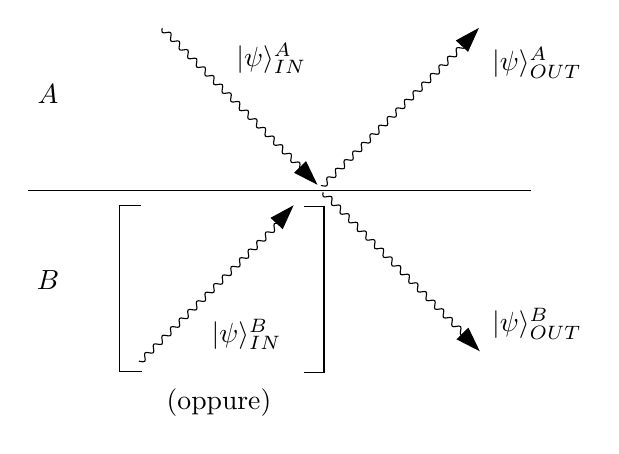
\begin{tikzpicture}[x=0.75pt,y=0.75pt,yscale=-1,xscale=1]
%uncomment if require: \path (0,300); %set diagram left start at 0, and has height of 300

%Straight Lines [id:da6800347625712677] 
\draw    (186.5,129.44) -- (428.75,129.44) ;


%Shape: Wave [id:dp43336901688240714] 
\draw   (250.98,51.44) .. controls (250.82,52.27) and (250.66,53.07) .. (251.04,53.45) .. controls (251.41,53.82) and (252.21,53.68) .. (253.05,53.52) .. controls (253.88,53.36) and (254.68,53.22) .. (255.06,53.59) .. controls (255.43,53.97) and (255.28,54.77) .. (255.12,55.6) .. controls (254.96,56.44) and (254.8,57.24) .. (255.18,57.61) .. controls (255.55,57.99) and (256.35,57.84) .. (257.19,57.69) .. controls (258.02,57.53) and (258.82,57.38) .. (259.2,57.76) .. controls (259.57,58.14) and (259.42,58.94) .. (259.26,59.77) .. controls (259.1,60.61) and (258.94,61.4) .. (259.32,61.78) .. controls (259.69,62.16) and (260.49,62.01) .. (261.33,61.86) .. controls (262.16,61.7) and (262.96,61.55) .. (263.34,61.93) .. controls (263.71,62.31) and (263.56,63.1) .. (263.4,63.94) .. controls (263.24,64.78) and (263.08,65.57) .. (263.46,65.95) .. controls (263.83,66.33) and (264.63,66.18) .. (265.47,66.02) .. controls (266.3,65.87) and (267.1,65.72) .. (267.48,66.1) .. controls (267.85,66.47) and (267.7,67.27) .. (267.54,68.11) .. controls (267.38,68.94) and (267.22,69.74) .. (267.6,70.12) .. controls (267.97,70.49) and (268.77,70.35) .. (269.61,70.19) .. controls (270.44,70.03) and (271.24,69.89) .. (271.62,70.26) .. controls (271.99,70.64) and (271.84,71.44) .. (271.68,72.27) .. controls (271.52,73.11) and (271.36,73.91) .. (271.74,74.28) .. controls (272.11,74.66) and (272.91,74.51) .. (273.75,74.36) .. controls (274.58,74.2) and (275.38,74.06) .. (275.76,74.43) .. controls (276.13,74.81) and (275.98,75.61) .. (275.82,76.44) .. controls (275.66,77.28) and (275.5,78.08) .. (275.88,78.45) .. controls (276.25,78.83) and (277.05,78.68) .. (277.89,78.53) .. controls (278.72,78.37) and (279.52,78.22) .. (279.9,78.6) .. controls (280.27,78.98) and (280.12,79.77) .. (279.96,80.61) .. controls (279.8,81.45) and (279.64,82.24) .. (280.02,82.62) .. controls (280.39,83) and (281.19,82.85) .. (282.03,82.69) .. controls (282.86,82.54) and (283.66,82.39) .. (284.04,82.77) .. controls (284.41,83.14) and (284.26,83.94) .. (284.1,84.78) .. controls (283.94,85.61) and (283.78,86.41) .. (284.16,86.79) .. controls (284.53,87.16) and (285.33,87.02) .. (286.17,86.86) .. controls (287,86.71) and (287.8,86.56) .. (288.18,86.94) .. controls (288.55,87.31) and (288.4,88.11) .. (288.24,88.95) .. controls (288.08,89.78) and (287.92,90.58) .. (288.3,90.95) .. controls (288.67,91.33) and (289.47,91.18) .. (290.31,91.03) .. controls (291.14,90.87) and (291.94,90.73) .. (292.32,91.1) .. controls (292.69,91.48) and (292.54,92.28) .. (292.38,93.11) .. controls (292.22,93.95) and (292.06,94.75) .. (292.44,95.12) .. controls (292.81,95.5) and (293.61,95.35) .. (294.45,95.2) .. controls (295.28,95.04) and (296.08,94.89) .. (296.46,95.27) .. controls (296.83,95.65) and (296.68,96.44) .. (296.52,97.28) .. controls (296.36,98.12) and (296.2,98.91) .. (296.58,99.29) .. controls (296.95,99.67) and (297.75,99.52) .. (298.59,99.36) .. controls (299.42,99.21) and (300.22,99.06) .. (300.6,99.44) .. controls (300.97,99.82) and (300.82,100.61) .. (300.66,101.45) .. controls (300.5,102.28) and (300.34,103.08) .. (300.72,103.46) .. controls (301.09,103.83) and (301.89,103.69) .. (302.73,103.53) .. controls (303.56,103.38) and (304.36,103.23) .. (304.74,103.61) .. controls (305.11,103.98) and (304.96,104.78) .. (304.8,105.62) .. controls (304.64,106.45) and (304.48,107.25) .. (304.86,107.63) .. controls (305.23,108) and (306.03,107.86) .. (306.87,107.7) .. controls (307.7,107.54) and (308.5,107.4) .. (308.88,107.77) .. controls (309.25,108.15) and (309.1,108.95) .. (308.94,109.78) .. controls (308.78,110.62) and (308.62,111.42) .. (309,111.79) .. controls (309.37,112.17) and (310.17,112.02) .. (311.01,111.87) .. controls (311.84,111.71) and (312.64,111.56) .. (313.02,111.94) .. controls (313.39,112.32) and (313.24,113.11) .. (313.08,113.95) .. controls (312.92,114.79) and (312.76,115.58) .. (313.14,115.96) .. controls (313.51,116.34) and (314.31,116.19) .. (315.15,116.03) .. controls (315.98,115.88) and (316.78,115.73) .. (317.16,116.11) .. controls (317.53,116.49) and (317.38,117.28) .. (317.22,118.12) .. controls (317.06,118.95) and (316.9,119.75) .. (317.28,120.13) .. controls (317.65,120.51) and (318.45,120.36) .. (319.29,120.2) .. controls (320.12,120.05) and (320.92,119.9) .. (321.3,120.28) .. controls (321.67,120.65) and (321.52,121.45) .. (321.36,122.29) .. controls (321.3,122.58) and (321.24,122.87) .. (321.21,123.14) ;
%Shape: Wave [id:dp6751405407771489] 
\draw   (398.97,56.78) .. controls (398.14,56.62) and (397.34,56.47) .. (396.96,56.84) .. controls (396.59,57.22) and (396.74,58.02) .. (396.9,58.85) .. controls (397.05,59.69) and (397.2,60.49) .. (396.83,60.86) .. controls (396.45,61.24) and (395.65,61.09) .. (394.82,60.93) .. controls (393.98,60.77) and (393.18,60.62) .. (392.81,60.99) .. controls (392.43,61.37) and (392.58,62.17) .. (392.74,63) .. controls (392.9,63.84) and (393.05,64.64) .. (392.67,65.01) .. controls (392.3,65.39) and (391.5,65.24) .. (390.66,65.08) .. controls (389.83,64.92) and (389.03,64.77) .. (388.65,65.15) .. controls (388.28,65.52) and (388.43,66.32) .. (388.58,67.15) .. controls (388.74,67.99) and (388.89,68.79) .. (388.52,69.16) .. controls (388.14,69.54) and (387.34,69.39) .. (386.51,69.23) .. controls (385.67,69.07) and (384.87,68.92) .. (384.5,69.3) .. controls (384.12,69.67) and (384.27,70.47) .. (384.43,71.31) .. controls (384.59,72.14) and (384.74,72.94) .. (384.36,73.32) .. controls (383.98,73.69) and (383.19,73.54) .. (382.35,73.38) .. controls (381.51,73.22) and (380.72,73.07) .. (380.34,73.45) .. controls (379.96,73.82) and (380.11,74.62) .. (380.27,75.46) .. controls (380.43,76.29) and (380.58,77.09) .. (380.2,77.47) .. controls (379.83,77.84) and (379.03,77.69) .. (378.19,77.53) .. controls (377.36,77.37) and (376.56,77.22) .. (376.18,77.6) .. controls (375.81,77.98) and (375.96,78.77) .. (376.12,79.61) .. controls (376.27,80.45) and (376.42,81.24) .. (376.05,81.62) .. controls (375.67,82) and (374.87,81.85) .. (374.04,81.69) .. controls (373.2,81.53) and (372.4,81.38) .. (372.03,81.75) .. controls (371.65,82.13) and (371.8,82.93) .. (371.96,83.76) .. controls (372.12,84.6) and (372.27,85.4) .. (371.89,85.77) .. controls (371.52,86.15) and (370.72,86) .. (369.88,85.84) .. controls (369.05,85.68) and (368.25,85.53) .. (367.87,85.9) .. controls (367.5,86.28) and (367.65,87.08) .. (367.8,87.91) .. controls (367.96,88.75) and (368.11,89.55) .. (367.74,89.92) .. controls (367.36,90.3) and (366.56,90.15) .. (365.73,89.99) .. controls (364.89,89.83) and (364.09,89.68) .. (363.72,90.06) .. controls (363.34,90.43) and (363.49,91.23) .. (363.65,92.06) .. controls (363.81,92.9) and (363.96,93.7) .. (363.58,94.07) .. controls (363.2,94.45) and (362.41,94.3) .. (361.57,94.14) .. controls (360.73,93.98) and (359.94,93.83) .. (359.56,94.21) .. controls (359.18,94.58) and (359.33,95.38) .. (359.49,96.22) .. controls (359.65,97.05) and (359.8,97.85) .. (359.42,98.23) .. controls (359.05,98.6) and (358.25,98.45) .. (357.41,98.29) .. controls (356.58,98.13) and (355.78,97.98) .. (355.4,98.36) .. controls (355.03,98.73) and (355.18,99.53) .. (355.34,100.37) .. controls (355.49,101.2) and (355.64,102) .. (355.27,102.38) .. controls (354.89,102.75) and (354.09,102.6) .. (353.26,102.44) .. controls (352.42,102.28) and (351.62,102.13) .. (351.25,102.51) .. controls (350.87,102.89) and (351.02,103.68) .. (351.18,104.52) .. controls (351.34,105.36) and (351.49,106.15) .. (351.11,106.53) .. controls (350.74,106.91) and (349.94,106.76) .. (349.1,106.6) .. controls (348.27,106.44) and (347.47,106.29) .. (347.09,106.66) .. controls (346.72,107.04) and (346.87,107.84) .. (347.02,108.67) .. controls (347.18,109.51) and (347.33,110.31) .. (346.96,110.68) .. controls (346.58,111.06) and (345.78,110.91) .. (344.95,110.75) .. controls (344.11,110.59) and (343.31,110.44) .. (342.94,110.81) .. controls (342.56,111.19) and (342.71,111.99) .. (342.87,112.82) .. controls (343.03,113.66) and (343.18,114.46) .. (342.8,114.83) .. controls (342.42,115.21) and (341.63,115.06) .. (340.79,114.9) .. controls (339.95,114.74) and (339.16,114.59) .. (338.78,114.97) .. controls (338.4,115.34) and (338.55,116.14) .. (338.71,116.97) .. controls (338.87,117.81) and (339.02,118.61) .. (338.64,118.98) .. controls (338.27,119.36) and (337.47,119.21) .. (336.63,119.05) .. controls (335.8,118.89) and (335,118.74) .. (334.62,119.12) .. controls (334.25,119.49) and (334.4,120.29) .. (334.56,121.13) .. controls (334.71,121.96) and (334.86,122.76) .. (334.49,123.14) .. controls (334.11,123.51) and (333.31,123.36) .. (332.48,123.2) .. controls (331.64,123.04) and (330.84,122.89) .. (330.47,123.27) .. controls (330.09,123.64) and (330.24,124.44) .. (330.4,125.28) .. controls (330.56,126.11) and (330.71,126.91) .. (330.33,127.29) .. controls (329.96,127.66) and (329.16,127.51) .. (328.32,127.35) .. controls (328.02,127.3) and (327.73,127.24) .. (327.46,127.21) ;
%Shape: Wave [id:dp4945236732065843] 
\draw   (328.52,130.49) .. controls (328.36,131.33) and (328.21,132.12) .. (328.58,132.5) .. controls (328.95,132.88) and (329.75,132.73) .. (330.59,132.57) .. controls (331.43,132.42) and (332.22,132.27) .. (332.6,132.65) .. controls (332.97,133.02) and (332.82,133.82) .. (332.66,134.66) .. controls (332.5,135.49) and (332.35,136.29) .. (332.72,136.67) .. controls (333.09,137.04) and (333.89,136.9) .. (334.73,136.74) .. controls (335.57,136.58) and (336.36,136.44) .. (336.74,136.81) .. controls (337.11,137.19) and (336.96,137.99) .. (336.8,138.82) .. controls (336.64,139.66) and (336.49,140.46) .. (336.86,140.83) .. controls (337.23,141.21) and (338.03,141.06) .. (338.87,140.91) .. controls (339.71,140.75) and (340.5,140.61) .. (340.88,140.98) .. controls (341.25,141.36) and (341.1,142.16) .. (340.94,142.99) .. controls (340.78,143.83) and (340.63,144.63) .. (341,145) .. controls (341.37,145.38) and (342.17,145.23) .. (343.01,145.08) .. controls (343.85,144.92) and (344.64,144.77) .. (345.02,145.15) .. controls (345.39,145.53) and (345.24,146.32) .. (345.08,147.16) .. controls (344.92,148) and (344.77,148.79) .. (345.14,149.17) .. controls (345.51,149.55) and (346.31,149.4) .. (347.15,149.24) .. controls (347.99,149.09) and (348.78,148.94) .. (349.16,149.32) .. controls (349.53,149.69) and (349.38,150.49) .. (349.22,151.33) .. controls (349.06,152.16) and (348.91,152.96) .. (349.28,153.34) .. controls (349.65,153.71) and (350.45,153.57) .. (351.29,153.41) .. controls (352.13,153.26) and (352.92,153.11) .. (353.3,153.49) .. controls (353.67,153.86) and (353.52,154.66) .. (353.36,155.5) .. controls (353.2,156.33) and (353.05,157.13) .. (353.42,157.51) .. controls (353.79,157.88) and (354.59,157.74) .. (355.43,157.58) .. controls (356.27,157.42) and (357.06,157.28) .. (357.44,157.65) .. controls (357.81,158.03) and (357.66,158.83) .. (357.5,159.66) .. controls (357.34,160.5) and (357.19,161.3) .. (357.56,161.67) .. controls (357.93,162.05) and (358.73,161.9) .. (359.57,161.75) .. controls (360.41,161.59) and (361.2,161.44) .. (361.58,161.82) .. controls (361.95,162.2) and (361.8,162.99) .. (361.64,163.83) .. controls (361.48,164.67) and (361.33,165.46) .. (361.7,165.84) .. controls (362.07,166.22) and (362.87,166.07) .. (363.71,165.91) .. controls (364.55,165.76) and (365.34,165.61) .. (365.72,165.99) .. controls (366.09,166.37) and (365.94,167.16) .. (365.78,168) .. controls (365.62,168.83) and (365.47,169.63) .. (365.84,170.01) .. controls (366.21,170.38) and (367.01,170.24) .. (367.85,170.08) .. controls (368.69,169.93) and (369.48,169.78) .. (369.86,170.16) .. controls (370.23,170.53) and (370.08,171.33) .. (369.92,172.17) .. controls (369.76,173) and (369.61,173.8) .. (369.98,174.18) .. controls (370.35,174.55) and (371.15,174.41) .. (371.99,174.25) .. controls (372.83,174.09) and (373.62,173.95) .. (374,174.32) .. controls (374.37,174.7) and (374.22,175.5) .. (374.06,176.33) .. controls (373.9,177.17) and (373.75,177.97) .. (374.12,178.34) .. controls (374.49,178.72) and (375.29,178.57) .. (376.13,178.42) .. controls (376.97,178.26) and (377.76,178.11) .. (378.14,178.49) .. controls (378.51,178.87) and (378.36,179.67) .. (378.2,180.5) .. controls (378.04,181.34) and (377.89,182.13) .. (378.26,182.51) .. controls (378.63,182.89) and (379.43,182.74) .. (380.27,182.58) .. controls (381.11,182.43) and (381.9,182.28) .. (382.28,182.66) .. controls (382.65,183.04) and (382.5,183.83) .. (382.34,184.67) .. controls (382.18,185.5) and (382.03,186.3) .. (382.4,186.68) .. controls (382.77,187.06) and (383.57,186.91) .. (384.41,186.75) .. controls (385.25,186.6) and (386.04,186.45) .. (386.42,186.83) .. controls (386.79,187.2) and (386.64,188) .. (386.48,188.84) .. controls (386.32,189.67) and (386.17,190.47) .. (386.54,190.85) .. controls (386.91,191.22) and (387.71,191.08) .. (388.55,190.92) .. controls (389.39,190.76) and (390.18,190.62) .. (390.56,190.99) .. controls (390.93,191.37) and (390.78,192.17) .. (390.62,193) .. controls (390.46,193.84) and (390.31,194.64) .. (390.68,195.01) .. controls (391.05,195.39) and (391.85,195.24) .. (392.69,195.09) .. controls (393.53,194.93) and (394.32,194.78) .. (394.7,195.16) .. controls (395.07,195.54) and (394.92,196.34) .. (394.76,197.17) .. controls (394.6,198.01) and (394.45,198.8) .. (394.82,199.18) .. controls (395.19,199.56) and (395.99,199.41) .. (396.83,199.25) .. controls (397.67,199.1) and (398.46,198.95) .. (398.84,199.33) .. controls (399.21,199.71) and (399.06,200.5) .. (398.9,201.34) .. controls (398.84,201.64) and (398.79,201.93) .. (398.75,202.2) ;
%Shape: Wave [id:dp6686945716273116] 
\draw   (311.21,141.39) .. controls (310.37,141.23) and (309.57,141.08) .. (309.2,141.46) .. controls (308.82,141.83) and (308.97,142.63) .. (309.13,143.47) .. controls (309.29,144.31) and (309.44,145.1) .. (309.06,145.48) .. controls (308.68,145.85) and (307.89,145.7) .. (307.05,145.54) .. controls (306.21,145.39) and (305.42,145.24) .. (305.04,145.61) .. controls (304.66,145.99) and (304.81,146.78) .. (304.97,147.62) .. controls (305.13,148.46) and (305.28,149.25) .. (304.9,149.63) .. controls (304.53,150.01) and (303.73,149.86) .. (302.89,149.7) .. controls (302.06,149.54) and (301.26,149.39) .. (300.88,149.76) .. controls (300.51,150.14) and (300.66,150.94) .. (300.82,151.77) .. controls (300.97,152.61) and (301.12,153.41) .. (300.75,153.78) .. controls (300.37,154.16) and (299.57,154.01) .. (298.74,153.85) .. controls (297.9,153.69) and (297.1,153.54) .. (296.73,153.91) .. controls (296.35,154.29) and (296.5,155.09) .. (296.66,155.92) .. controls (296.82,156.76) and (296.97,157.56) .. (296.59,157.93) .. controls (296.22,158.31) and (295.42,158.16) .. (294.58,158) .. controls (293.75,157.84) and (292.95,157.69) .. (292.57,158.07) .. controls (292.2,158.44) and (292.35,159.24) .. (292.5,160.08) .. controls (292.66,160.91) and (292.81,161.71) .. (292.44,162.09) .. controls (292.06,162.46) and (291.26,162.31) .. (290.43,162.15) .. controls (289.59,161.99) and (288.79,161.84) .. (288.42,162.22) .. controls (288.04,162.59) and (288.19,163.39) .. (288.35,164.23) .. controls (288.51,165.06) and (288.66,165.86) .. (288.28,166.24) .. controls (287.9,166.61) and (287.11,166.46) .. (286.27,166.3) .. controls (285.43,166.14) and (284.64,165.99) .. (284.26,166.37) .. controls (283.88,166.74) and (284.03,167.54) .. (284.19,168.38) .. controls (284.35,169.22) and (284.5,170.01) .. (284.12,170.39) .. controls (283.75,170.76) and (282.95,170.61) .. (282.11,170.45) .. controls (281.28,170.3) and (280.48,170.15) .. (280.1,170.52) .. controls (279.73,170.9) and (279.88,171.69) .. (280.04,172.53) .. controls (280.19,173.37) and (280.34,174.16) .. (279.97,174.54) .. controls (279.59,174.92) and (278.79,174.77) .. (277.96,174.61) .. controls (277.12,174.45) and (276.32,174.3) .. (275.95,174.67) .. controls (275.57,175.05) and (275.72,175.85) .. (275.88,176.68) .. controls (276.04,177.52) and (276.19,178.32) .. (275.81,178.69) .. controls (275.44,179.07) and (274.64,178.92) .. (273.8,178.76) .. controls (272.97,178.6) and (272.17,178.45) .. (271.79,178.82) .. controls (271.42,179.2) and (271.57,180) .. (271.72,180.83) .. controls (271.88,181.67) and (272.03,182.47) .. (271.66,182.84) .. controls (271.28,183.22) and (270.48,183.07) .. (269.65,182.91) .. controls (268.81,182.75) and (268.01,182.6) .. (267.64,182.98) .. controls (267.26,183.35) and (267.41,184.15) .. (267.57,184.99) .. controls (267.73,185.82) and (267.88,186.62) .. (267.5,187) .. controls (267.12,187.37) and (266.33,187.22) .. (265.49,187.06) .. controls (264.65,186.9) and (263.86,186.75) .. (263.48,187.13) .. controls (263.1,187.5) and (263.25,188.3) .. (263.41,189.14) .. controls (263.57,189.97) and (263.72,190.77) .. (263.34,191.15) .. controls (262.97,191.52) and (262.17,191.37) .. (261.33,191.21) .. controls (260.5,191.05) and (259.7,190.9) .. (259.32,191.28) .. controls (258.95,191.65) and (259.1,192.45) .. (259.26,193.29) .. controls (259.41,194.13) and (259.56,194.92) .. (259.19,195.3) .. controls (258.81,195.67) and (258.01,195.52) .. (257.18,195.36) .. controls (256.34,195.21) and (255.54,195.06) .. (255.17,195.43) .. controls (254.79,195.81) and (254.94,196.6) .. (255.1,197.44) .. controls (255.26,198.28) and (255.41,199.07) .. (255.03,199.45) .. controls (254.66,199.83) and (253.86,199.68) .. (253.02,199.52) .. controls (252.19,199.36) and (251.39,199.21) .. (251.01,199.58) .. controls (250.64,199.96) and (250.79,200.76) .. (250.94,201.59) .. controls (251.1,202.43) and (251.25,203.23) .. (250.88,203.6) .. controls (250.5,203.98) and (249.7,203.83) .. (248.87,203.67) .. controls (248.03,203.51) and (247.23,203.36) .. (246.86,203.73) .. controls (246.48,204.11) and (246.63,204.91) .. (246.79,205.74) .. controls (246.95,206.58) and (247.1,207.38) .. (246.72,207.75) .. controls (246.34,208.13) and (245.55,207.98) .. (244.71,207.82) .. controls (243.87,207.66) and (243.08,207.51) .. (242.7,207.89) .. controls (242.32,208.26) and (242.47,209.06) .. (242.63,209.9) .. controls (242.79,210.73) and (242.94,211.53) .. (242.56,211.91) .. controls (242.19,212.28) and (241.39,212.13) .. (240.55,211.97) .. controls (240.26,211.91) and (239.96,211.86) .. (239.69,211.83) ;
%Shape: Triangle [id:dp24906687948860196] 
\draw  [color={rgb, 255:red, 0; green, 0; blue, 0 }  ,draw opacity=1 ][fill={rgb, 255:red, 0; green, 0; blue, 0 }  ,fill opacity=1 ] (325.2,126.26) -- (314.98,121.02) -- (320.2,115.91) -- cycle ;
%Shape: Triangle [id:dp9532617638179957] 
\draw  [color={rgb, 255:red, 0; green, 0; blue, 0 }  ,draw opacity=1 ][fill={rgb, 255:red, 0; green, 0; blue, 0 }  ,fill opacity=1 ] (403.42,206.49) -- (393.19,201.24) -- (398.42,196.14) -- cycle ;
%Shape: Triangle [id:dp05587931334957452] 
\draw  [color={rgb, 255:red, 0; green, 0; blue, 0 }  ,draw opacity=1 ][fill={rgb, 255:red, 0; green, 0; blue, 0 }  ,fill opacity=1 ] (402.99,51.91) -- (398.23,62.37) -- (392.89,57.39) -- cycle ;
%Shape: Triangle [id:dp9662989558108341] 
\draw  [color={rgb, 255:red, 0; green, 0; blue, 0 }  ,draw opacity=1 ][fill={rgb, 255:red, 0; green, 0; blue, 0 }  ,fill opacity=1 ] (313.71,137.37) -- (308.95,147.83) -- (303.61,142.85) -- cycle ;
%Straight Lines [id:da05459906991776453] 
\draw    (240.58,136.83) -- (230.58,136.83) -- (230.58,216.83) -- (241.25,216.83) ;


%Straight Lines [id:da15655694257834707] 
\draw    (319.42,137.17) -- (328.92,137.17) -- (328.92,217.17) -- (319.08,217.17) ;



% Text Node
\draw (196,83) node   {$A$};
% Text Node
\draw (196,173) node   {$B$};
% Text Node
\draw (291.6,198.9) node   {$|\psi \rangle ^{B}_{IN}$};
% Text Node
\draw (303.5,66) node   {$|\psi \rangle ^{A}_{IN}$};
% Text Node
\draw (431.5,68) node   {$|\psi \rangle ^{A}_{OUT}$};
% Text Node
\draw (431.5,194) node   {$|\psi \rangle ^{B}_{OUT}$};
% Text Node
\draw (278.33,232) node  [align=left] {(oppure)};


\end{tikzpicture}
\end{center}
\caption{Schema del funzionamento del Beam Splitter.
\label{fig:beam-splitter}}
\end{figure}
L'effetto di un beam-splitter può essere schematizzato come quello di un opportuno \textbf{gate quantistico} $U_{B.S.}$, tale che:
\begin{align*}
\ket{1}^A_{in}\ket{0}^B_{in} \xrightarrow{U_{B.S.}} \frac{1}{\sqrt{2}}\ket{1}^A_{out} \ket{0}^B_{out} + \frac{i}{\sqrt{2}}\ket{0}^A_{out}\ket{1}^B_{out}
\end{align*}
Per cui un fotone che arriva da \textit{fuori} (cioè da $A$) può essere rimandato fuori (di nuovo in $A$) o dentro (in $B$), con ugual probabilità. Nel caso di \textbf{trasmissione} il fotone acquisisce una fase $i$ (cioè di $\pi/2$).\\
Vale la relazione analoga nel caso un fotone arrivi \q{da dentro}, ossia da $B$:
\begin{align*}
\ket{0}^A_{in}\ket{1}^B_{in} \xrightarrow{U_{B.S.}} \frac{i}{\sqrt{2}}\ket{1}^A_{out}\ket{0}^B_{out} + \frac{1}{\sqrt{2}}\ket{0}^A_{out}\ket{1}^B_{out}
\end{align*}
Possiamo sintetizzare queste due relazioni scrivendo $U_{BS}$ in notazione matriciale nella base $\{\ket{1}^A \ket{0}^B, \ket{0}^A \ket{1}^B \}$:
\begin{align*}
\ket{\psi_{out}} = \frac{1}{\sqrt{2}}\begin{pmatrix}1 & i\\i & 1\end{pmatrix}\ket{\psi_{in}}
\end{align*}
\end{itemize}

\subsection{Interferometro di Mach-Zehnder quantistico}
Un modo per effettuare una misura senza interazione avviene tramite l'uso di un \textbf{interferometro di Mach-Zehnder}\index{Interferometro di Mach-Zehnder}, rappresentato in figura \ref{fig:interferometro}.

\begin{figure}[H]
\centering


\tikzset{every picture/.style={line width=0.75pt}} %set default line width to 0.75pt        
\begin{center}
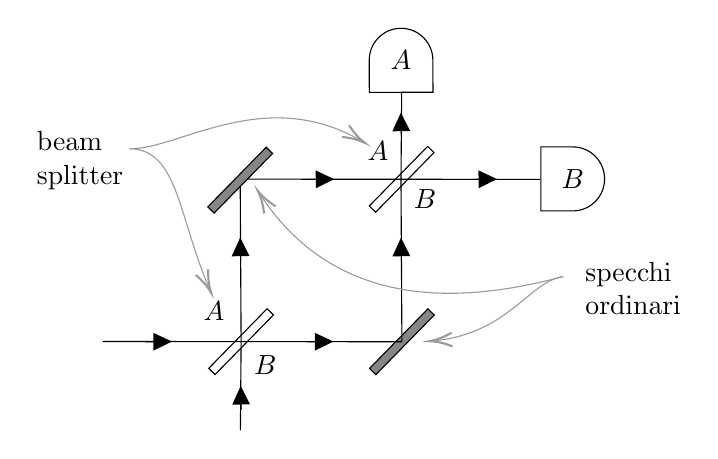
\begin{tikzpicture}[x=0.75pt,y=0.75pt,yscale=-1,xscale=1]
%uncomment if require: \path (0,300); %set diagram left start at 0, and has height of 300

%Shape: Rectangle [id:dp03258470004560032] 
\draw   (314.64,178.14) -- (342.76,149.42) -- (345.8,152.43) -- (317.68,181.15) -- cycle ;
%Straight Lines [id:da6232747865539225] 
\draw    (330.22,165.29) -- (329.88,208) ;


%Straight Lines [id:da7516321880556363] 
\draw    (263.51,165.2) -- (330.22,165.29) ;


%Straight Lines [id:da7431820818677963] 
\draw    (329.78,87.5) -- (330.22,165.29) ;


%Shape: Rectangle [id:dp9234193027203714] 
\draw  [color={rgb, 255:red, 0; green, 0; blue, 0 }  ,draw opacity=1 ][fill={rgb, 255:red, 134; green, 134; blue, 134 }  ,fill opacity=1 ] (392.11,178.18) -- (420.24,149.46) -- (423.28,152.47) -- (395.15,181.19) -- cycle ;
%Shape: Rectangle [id:dp45539842012124043] 
\draw   (392,99.91) -- (420.13,71.19) -- (423.17,74.2) -- (395.05,102.92) -- cycle ;
%Straight Lines [id:da41484953628459365] 
\draw    (330.22,165.29) -- (407.69,165.33) ;


%Straight Lines [id:da6769463633535804] 
\draw    (330.11,87.01) -- (407.59,87.05) ;


%Straight Lines [id:da3686137129912357] 
\draw    (407.25,87.53) -- (407.69,165.33) ;


%Straight Lines [id:da2517530051922354] 
\draw    (407.59,87.05) -- (474.29,87.14) ;


%Straight Lines [id:da24300038090025722] 
\draw    (407.59,44.82) -- (407.25,87.53) ;


%Shape: Rectangle [id:dp1865303790271311] 
\draw  [color={rgb, 255:red, 0; green, 0; blue, 0 }  ,draw opacity=1 ][fill={rgb, 255:red, 134; green, 134; blue, 134 }  ,fill opacity=1 ] (314.19,100.35) -- (342.32,71.63) -- (345.36,74.64) -- (317.23,103.36) -- cycle ;
%Straight Lines [id:da2941942939542457] 
\draw    (284.27,165.35) -- (294.87,165.26) ;
\draw [shift={(296.87,165.24)}, rotate = 539.49] [fill={rgb, 255:red, 0; green, 0; blue, 0 }  ][line width=0.75]  [draw opacity=0] (8.93,-4.29) -- (0,0) -- (8.93,4.29) -- cycle    ;

%Straight Lines [id:da5296598357878515] 
\draw    (330.27,197.87) -- (330.09,188.64) ;
\draw [shift={(330.05,186.64)}, rotate = 448.87] [fill={rgb, 255:red, 0; green, 0; blue, 0 }  ][line width=0.75]  [draw opacity=0] (8.93,-4.29) -- (0,0) -- (8.93,4.29) -- cycle    ;

%Straight Lines [id:da8396982575668597] 
\draw    (330,126.39) -- (329.82,117.17) ;
\draw [shift={(329.78,115.17)}, rotate = 448.87] [fill={rgb, 255:red, 0; green, 0; blue, 0 }  ][line width=0.75]  [draw opacity=0] (8.93,-4.29) -- (0,0) -- (8.93,4.29) -- cycle    ;

%Straight Lines [id:da43067332906978706] 
\draw    (362.08,165.35) -- (372.68,165.26) ;
\draw [shift={(374.68,165.24)}, rotate = 539.49] [fill={rgb, 255:red, 0; green, 0; blue, 0 }  ][line width=0.75]  [draw opacity=0] (8.93,-4.29) -- (0,0) -- (8.93,4.29) -- cycle    ;

%Straight Lines [id:da3506455513682578] 
\draw    (407.47,126.43) -- (407.29,117.2) ;
\draw [shift={(407.25,115.21)}, rotate = 448.87] [fill={rgb, 255:red, 0; green, 0; blue, 0 }  ][line width=0.75]  [draw opacity=0] (8.93,-4.29) -- (0,0) -- (8.93,4.29) -- cycle    ;

%Straight Lines [id:da5029542426839855] 
\draw    (362.52,87.12) -- (373.12,87.02) ;
\draw [shift={(375.12,87.01)}, rotate = 539.49] [fill={rgb, 255:red, 0; green, 0; blue, 0 }  ][line width=0.75]  [draw opacity=0] (8.93,-4.29) -- (0,0) -- (8.93,4.29) -- cycle    ;

%Straight Lines [id:da08573326322161745] 
\draw    (440.94,87.1) -- (451.54,87) ;
\draw [shift={(453.54,86.99)}, rotate = 539.49] [fill={rgb, 255:red, 0; green, 0; blue, 0 }  ][line width=0.75]  [draw opacity=0] (8.93,-4.29) -- (0,0) -- (8.93,4.29) -- cycle    ;

%Straight Lines [id:da9310563696791143] 
\draw    (407.42,66.18) -- (407.24,56.95) ;
\draw [shift={(407.2,54.95)}, rotate = 448.87] [fill={rgb, 255:red, 0; green, 0; blue, 0 }  ][line width=0.75]  [draw opacity=0] (8.93,-4.29) -- (0,0) -- (8.93,4.29) -- cycle    ;

%Flowchart: Delay [id:dp15978253790159513] 
\draw   (474.67,71.47) -- (490.01,71.47) .. controls (498.48,71.47) and (505.34,78.38) .. (505.34,86.89) .. controls (505.34,95.41) and (498.48,102.31) .. (490.01,102.31) -- (474.67,102.31) -- cycle ;
%Flowchart: Delay [id:dp7496896065211829] 
\draw   (391.99,45.21) -- (391.94,29.79) .. controls (391.91,21.28) and (398.75,14.35) .. (407.22,14.32) .. controls (415.69,14.29) and (422.58,21.17) .. (422.61,29.69) -- (422.66,45.11) -- cycle ;
%Curve Lines [id:da1551059930194223] 
\draw [color={rgb, 255:red, 155; green, 154; blue, 154 }  ,draw opacity=1 ]   (485.48,133.93) .. controls (468.93,136.12) and (459.25,161.6) .. (422.63,164.92) ;
\draw [shift={(420.93,165.05)}, rotate = 355.99] [color={rgb, 255:red, 155; green, 154; blue, 154 }  ,draw opacity=1 ][line width=0.75]    (10.93,-3.29) .. controls (6.95,-1.4) and (3.31,-0.3) .. (0,0) .. controls (3.31,0.3) and (6.95,1.4) .. (10.93,3.29)   ;

%Curve Lines [id:da20331933767853982] 
\draw [color={rgb, 255:red, 155; green, 154; blue, 154 }  ,draw opacity=1 ]   (485.48,133.93) .. controls (446.77,144.11) and (378.73,155.6) .. (338.86,93.54) ;
\draw [shift={(338.26,92.59)}, rotate = 417.77] [color={rgb, 255:red, 155; green, 154; blue, 154 }  ,draw opacity=1 ][line width=0.75]    (10.93,-3.29) .. controls (6.95,-1.4) and (3.31,-0.3) .. (0,0) .. controls (3.31,0.3) and (6.95,1.4) .. (10.93,3.29)   ;

%Curve Lines [id:da4920771230228518] 
\draw [color={rgb, 255:red, 155; green, 154; blue, 154 }  ,draw opacity=1 ]   (276.56,72.31) .. controls (299.96,72.86) and (299.78,104.67) .. (315.08,140.14) ;
\draw [shift={(315.79,141.77)}, rotate = 246.07] [color={rgb, 255:red, 155; green, 154; blue, 154 }  ,draw opacity=1 ][line width=0.75]    (10.93,-3.29) .. controls (6.95,-1.4) and (3.31,-0.3) .. (0,0) .. controls (3.31,0.3) and (6.95,1.4) .. (10.93,3.29)   ;

%Curve Lines [id:da3557276256319264] 
\draw [color={rgb, 255:red, 155; green, 154; blue, 154 }  ,draw opacity=1 ]   (276.56,72.31) .. controls (300.08,72.86) and (341.48,41.28) .. (388.42,68.68) ;
\draw [shift={(389.84,69.53)}, rotate = 211.3] [color={rgb, 255:red, 155; green, 154; blue, 154 }  ,draw opacity=1 ][line width=0.75]    (10.93,-3.29) .. controls (6.95,-1.4) and (3.31,-0.3) .. (0,0) .. controls (3.31,0.3) and (6.95,1.4) .. (10.93,3.29)   ;


% Text Node
\draw (341.93,176.77) node   {$B$};
% Text Node
\draw (317.17,150.66) node   {$A$};
% Text Node
\draw (396.2,73.42) node   {$A$};
% Text Node
\draw (418.86,96.76) node   {$B$};
% Text Node
\draw (519.11,139.77) node  [align=left] {specchi\\ordinari};
% Text Node
\draw (252.63,78.09) node  [align=left] {beam\\splitter};
% Text Node
\draw (490.01,86.89) node   {$B$};
% Text Node
\draw (407.27,29.74) node   {$A$};


\end{tikzpicture}
\end{center}
\caption{Schema dell'interferometro di Mach-Zehnder.
\label{fig:interferometro}}
\end{figure}

Consideriamo un fotone che parte da $A$. Al primo passaggio attraverso il \textit{beam-splitter} avremo con $p=1/2$ una riflessione verso l'alto e con $p=1/2$ una trasmissione verso destra $B$. In entrambi i casi il fotone incide poi contro un normale specchio, e viene riflesso verso il secondo \textit{beam-splitter}. In \MQ entrambi i percorsi sono esplorati contemporaneamente, e interferiscono tra loro al ricongiungimento nel secondo \textit{BS}.\\

Innanzitutto, in entrambi i percorsi si ha una riflessione su uno specchio normale, che introduce in ciascun caso una fase\footnote{Dato che il materiale riflettente ha un indice di rifrazione per forza maggiore di quello del vuoto} $\pi$, senza però variare la differenza tra le fasi delle due \q{versioni} del fotone: possiamo perciò trascurare questo dettaglio. Percorriamo allora il circuito, seguendo i due possibili percorsi, partendo da un fotone che inizialmente è \q{in fase con se stesso}:  
\begin{itemize}
\item Se il fotone viene inizialmente riflesso dal primo BS, allora non acquisisce nessuna fase. Dopo aver oltrepassato il secondo BS, avremo quindi una possibilità con fase $1$ ($\theta = 0$) appena prima del detector in $A$, dovuta ad una seconda riflessione sul BS, e una con fase ancora $i$ prima del detector $B$, prodotta dalla trasmissione attraverso il BS.
\item Se il fotone viene trasmesso dal primo BS, allora arriva al secondo con una fase $i$. A questo punto, per raggiungere il detector $A$ deve essere nuovamente trasmesso attraverso il BS, acquisendo un'ulteriore fase $i$ e arrivando ad una fase totale $i^2$. Se invece viene riflesso verso il detector $B$ mantiene la sua fase di $i$.
\end{itemize}
Notiamo allora che prima del detector $A$, due versioni dello stesso fotone con \textit{fase opposta} ($i^2 = -1$, e $1$) interagiscono tra loro in modo \textit{distruttivo}, e quindi il rivelatore in $A$ non troverà alcun segnale.\\
D'altro canto, davanti a $B$ le \q{due versioni del fotone} interagiscono con la \textit{stessa fase} $i$, e quindi avremo \textit{interferenza costruttiva} e il rivelatore $B$ osserverà \textbf{sempre} la presenza del fotone.\\

In maniera analoga si può ricavare il funzionamento nel caso il fotone parta da $B$ e non da $A$, ottenendo una $p=1$ di rivelazione al detector $A$.\\

Un modo più semplice per capire tutto ciò è schematizzare l'interferometro come l'applicazione consecutiva di due gate $U_{BS}$, come mostrato in figura \ref{fig:circuito-B.S}.

\begin{figure}[H]
\centering


\tikzset{every picture/.style={line width=0.75pt}} %set default line width to 0.75pt        
\begin{center}
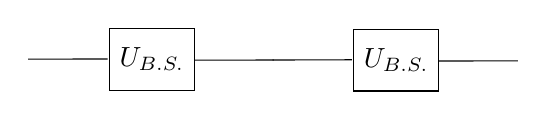
\begin{tikzpicture}[x=0.75pt,y=0.75pt,yscale=-1,xscale=1]
%uncomment if require: \path (0,300); %set diagram left start at 0, and has height of 300

%Straight Lines [id:da10643084520739499] 
\draw    (260.9,210.18) -- (299.14,210.07) ;


%Shape: Rectangle [id:dp7371746860618467] 
\draw   (299.95,195.27) -- (341.01,195.27) -- (341.01,225.1) -- (299.95,225.1) -- cycle ;
%Straight Lines [id:da7175370384571684] 
\draw    (340.94,210.67) -- (379.14,210.58) ;


%Straight Lines [id:da2619549169513742] 
\draw    (378.6,210.58) -- (416.84,210.47) ;


%Shape: Rectangle [id:dp6227610007372693] 
\draw   (417.65,195.67) -- (458.7,195.67) -- (458.7,225.5) -- (417.65,225.5) -- cycle ;
%Straight Lines [id:da14706233086125264] 
\draw    (458.64,211.07) -- (496.83,210.98) ;



% Text Node
\draw (320.48,210.18) node   {$U_{B.S.}$};
% Text Node
\draw (438.18,210.58) node   {$U_{B.S.}$};


\end{tikzpicture}
\end{center}
\caption{Schema con porte logiche quantistiche dell'interferometro di Mach-Zehnder.\label{fig:circuito-B.S}}
\end{figure}

Effettuando allora la computazione passo a passo:
\begin{align*}
\ket{0} \xrightarrow{U_{BS}} \frac{\ket{0}+i\ket{1}}{\sqrt{2}} \xrightarrow{U_{BS}} \frac{1}{2}\left[\ket{0}+i\ket{1}+i(i\ket{0}+\ket{1})\right] = i\ket{1}
\end{align*}

Alternativamente si ottiene lo stesso risultato calcolando il quadrato della matrice di $U_{BS}$:
\begin{align*}
U_{BS}^2 = \begin{pmatrix}
0 & i\\i & 0
\end{pmatrix}
\end{align*}

\begin{comment}
\textbf{Q.A.}
\begin{itemize}
\item Una CNOT \textbf{non} effettua una misura sul bit di controllo, ma instaura una correlazione \textit{senza modificarne} lo stato quantistico
\item Si può invertire l'ordine dei gate in un circuito quantistico senza cambiare l'operatore che esso rappresenta se e solo se tali operatori commutano tra loro (nell'esempio dell'esercizio 2 della scorsa volta succede, ma è un caso particolare)
\item Prova a cercare la rappresentazione della CPHASE in termini delle altre porte logiche (CNOT e phase shift)
\end{itemize}
\end{comment}

\subsection{Il test della bomba di Elitzur–Vaidman}
Siamo partiti dicendo che, tramite l'interferometro di Mach-Zehnder, risulta possibile effettuare una misura senza interazione. Vediamo allora come fare, con un esempio \textit{fortemente drammatico}.\index{Elitzur-Vaidman bomb tester}\\
Un terrorista ha costruito una \textit{bomba}, dotandola di un detonatore che può essere attivato dall'interazione con un \textit{singolo fotone}. Tale bomba è nascosta in una scatola trasparente, che viene posta lungo il cammino dell'interferometro di Mach-Zehnder (figura \ref{fig:interferometro-bomba}), ma a priori non sappiamo se si tratti di un \textit{bluff} (cioè di una scatola vuota) o di un effettivo pericolo (la scatola contiene la bomba). Scopo dell'esperimento è distinguere i due casi \textit{senza attivare la bomba}.

\begin{figure}[H]
\centering


\tikzset{every picture/.style={line width=0.75pt}} %set default line width to 0.75pt        
\begin{center}
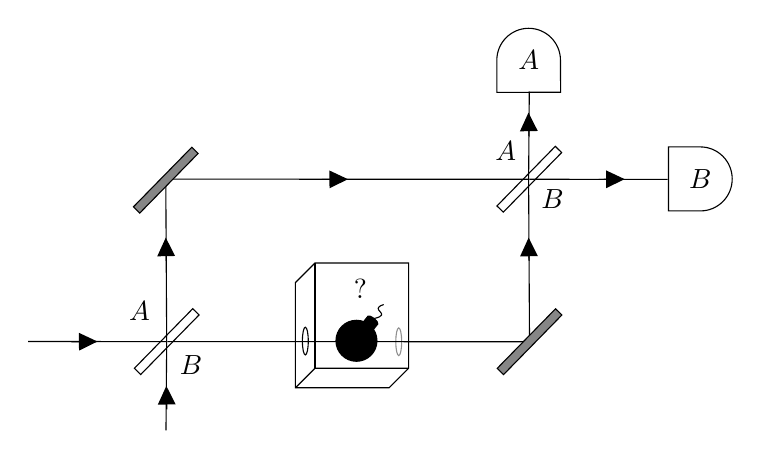
\begin{tikzpicture}[x=0.75pt,y=0.75pt,yscale=-1,xscale=1]
%uncomment if require: \path (0,300); %set diagram left start at 0, and has height of 300

%Shape: Rectangle [id:dp05331443244256162] 
\draw   (232.64,194.14) -- (260.76,165.42) -- (263.8,168.43) -- (235.68,197.15) -- cycle ;
%Straight Lines [id:da6101932312929839] 
\draw    (248.22,181.29) -- (247.88,224) ;


%Straight Lines [id:da37500240484008773] 
\draw    (181.51,181.2) -- (248.22,181.29) ;


%Straight Lines [id:da7395900492947349] 
\draw    (247.78,103.5) -- (248.22,181.29) ;


%Shape: Rectangle [id:dp7145865786703387] 
\draw   (407.34,115.91) -- (435.46,87.19) -- (438.5,90.2) -- (410.38,118.92) -- cycle ;
%Straight Lines [id:da406692659919365] 
\draw    (248.58,181.29) -- (423.03,181.33) ;


%Straight Lines [id:da251128727045983] 
\draw    (248.33,103.01) -- (422.78,103.05) ;


%Straight Lines [id:da6635342486103979] 
\draw    (422.59,103.53) -- (423.03,181.33) ;


%Straight Lines [id:da7433774894582017] 
\draw    (422.92,103.05) -- (489.62,103.14) ;


%Straight Lines [id:da6227633326802493] 
\draw    (422.92,60.82) -- (422.59,103.53) ;


%Shape: Rectangle [id:dp9484177753358207] 
\draw  [color={rgb, 255:red, 0; green, 0; blue, 0 }  ,draw opacity=1 ][fill={rgb, 255:red, 134; green, 134; blue, 134 }  ,fill opacity=1 ] (232.19,116.35) -- (260.32,87.63) -- (263.36,90.64) -- (235.23,119.36) -- cycle ;
%Straight Lines [id:da9162790812582262] 
\draw    (202.27,181.35) -- (212.87,181.26) ;
\draw [shift={(214.87,181.24)}, rotate = 539.49] [fill={rgb, 255:red, 0; green, 0; blue, 0 }  ][line width=0.75]  [draw opacity=0] (8.93,-4.29) -- (0,0) -- (8.93,4.29) -- cycle    ;

%Straight Lines [id:da6345146939842947] 
\draw    (248.27,213.87) -- (248.09,204.64) ;
\draw [shift={(248.05,202.64)}, rotate = 448.87] [fill={rgb, 255:red, 0; green, 0; blue, 0 }  ][line width=0.75]  [draw opacity=0] (8.93,-4.29) -- (0,0) -- (8.93,4.29) -- cycle    ;

%Straight Lines [id:da5741704284114686] 
\draw    (248,142.39) -- (247.82,133.17) ;
\draw [shift={(247.78,131.17)}, rotate = 448.87] [fill={rgb, 255:red, 0; green, 0; blue, 0 }  ][line width=0.75]  [draw opacity=0] (8.93,-4.29) -- (0,0) -- (8.93,4.29) -- cycle    ;

%Straight Lines [id:da9412424001460007] 
\draw    (422.81,142.43) -- (422.63,133.2) ;
\draw [shift={(422.59,131.21)}, rotate = 448.87] [fill={rgb, 255:red, 0; green, 0; blue, 0 }  ][line width=0.75]  [draw opacity=0] (8.93,-4.29) -- (0,0) -- (8.93,4.29) -- cycle    ;

%Straight Lines [id:da16868581259330884] 
\draw    (322.96,103.14) -- (333.56,103.05) ;
\draw [shift={(335.56,103.03)}, rotate = 539.49] [fill={rgb, 255:red, 0; green, 0; blue, 0 }  ][line width=0.75]  [draw opacity=0] (8.93,-4.29) -- (0,0) -- (8.93,4.29) -- cycle    ;

%Straight Lines [id:da32815921714688745] 
\draw    (456.27,103.1) -- (466.87,103) ;
\draw [shift={(468.87,102.99)}, rotate = 539.49] [fill={rgb, 255:red, 0; green, 0; blue, 0 }  ][line width=0.75]  [draw opacity=0] (8.93,-4.29) -- (0,0) -- (8.93,4.29) -- cycle    ;

%Straight Lines [id:da5754252869558345] 
\draw    (422.75,82.18) -- (422.57,72.95) ;
\draw [shift={(422.53,70.95)}, rotate = 448.87] [fill={rgb, 255:red, 0; green, 0; blue, 0 }  ][line width=0.75]  [draw opacity=0] (8.93,-4.29) -- (0,0) -- (8.93,4.29) -- cycle    ;

%Flowchart: Delay [id:dp9432596481685707] 
\draw   (490.01,87.47) -- (505.34,87.47) .. controls (513.81,87.47) and (520.68,94.38) .. (520.68,102.89) .. controls (520.68,111.41) and (513.81,118.31) .. (505.34,118.31) -- (490.01,118.31) -- cycle ;
%Flowchart: Delay [id:dp4563574851197332] 
\draw   (407.32,61.21) -- (407.27,45.79) .. controls (407.24,37.28) and (414.08,30.35) .. (422.55,30.32) .. controls (431.02,30.29) and (437.91,37.17) .. (437.94,45.69) -- (438,61.11) -- cycle ;
%Shape: Rectangle [id:dp6254395580176015] 
\draw  [color={rgb, 255:red, 0; green, 0; blue, 0 }  ,draw opacity=1 ][fill={rgb, 255:red, 134; green, 134; blue, 134 }  ,fill opacity=1 ] (407.45,194.18) -- (435.57,165.46) -- (438.61,168.47) -- (410.49,197.19) -- cycle ;
%Shape: Circle [id:dp013195896602818946] 
\draw  [fill={rgb, 255:red, 0; green, 0; blue, 0 }  ,fill opacity=1 ] (329.77,180.88) .. controls (329.77,175.42) and (334.19,171) .. (339.64,171) .. controls (345.1,171) and (349.52,175.42) .. (349.52,180.88) .. controls (349.52,186.33) and (345.1,190.75) .. (339.64,190.75) .. controls (334.19,190.75) and (329.77,186.33) .. (329.77,180.88) -- cycle ;
%Flowchart: Stored Data [id:dp9468842845409164] 
\draw  [fill={rgb, 255:red, 0; green, 0; blue, 0 }  ,fill opacity=1 ] (349.91,172.79) -- (346.81,176.69) .. controls (347.14,176.28) and (346.34,175.11) .. (345.04,174.07) .. controls (343.74,173.04) and (342.42,172.53) .. (342.09,172.94) -- (345.19,169.04) .. controls (345.51,168.63) and (346.84,169.14) .. (348.14,170.17) .. controls (349.44,171.21) and (350.24,172.38) .. (349.91,172.79) -- cycle ;
%Curve Lines [id:da5409664000175873] 
\draw    (348.14,170.17) .. controls (357.52,167.92) and (345.02,165.92) .. (352.77,163.42) ;


%Shape: Cube [id:dp23004251794331032] 
\draw   (364.78,194.13) -- (355.37,203.53) -- (310.25,203.53) -- (310.25,152.81) -- (319.66,143.4) -- (364.78,143.4) -- cycle ; \draw   (310.25,203.53) -- (319.66,194.13) -- (364.78,194.13) ; \draw   (319.66,194.13) -- (319.66,143.4) ;
%Shape: Ellipse [id:dp3375854777763616] 
\draw   (313.6,181) .. controls (313.6,177.32) and (314.23,174.33) .. (315.02,174.33) .. controls (315.8,174.33) and (316.43,177.32) .. (316.43,181) .. controls (316.43,184.68) and (315.8,187.67) .. (315.02,187.67) .. controls (314.23,187.67) and (313.6,184.68) .. (313.6,181) -- cycle ;
%Shape: Ellipse [id:dp1573514547024959] 
\draw  [color={rgb, 255:red, 0; green, 0; blue, 0 }  ,draw opacity=0.44 ][fill={rgb, 255:red, 0; green, 0; blue, 0 }  ,fill opacity=0 ] (358.6,181.33) .. controls (358.6,177.65) and (359.23,174.67) .. (360.02,174.67) .. controls (360.8,174.67) and (361.43,177.65) .. (361.43,181.33) .. controls (361.43,185.02) and (360.8,188) .. (360.02,188) .. controls (359.23,188) and (358.6,185.02) .. (358.6,181.33) -- cycle ;

% Text Node
\draw (259.93,192.77) node   {$B$};
% Text Node
\draw (235.17,166.66) node   {$A$};
% Text Node
\draw (411.53,89.42) node   {$A$};
% Text Node
\draw (434.19,112.76) node   {$B$};
% Text Node
\draw (505.34,102.89) node   {$B$};
% Text Node
\draw (422.61,45.74) node   {$A$};
% Text Node
\draw (341.6,156) node  [align=left] {?};


\end{tikzpicture}
\end{center}
\caption{Interferometro di Mach-Zehnder utilizzato per misure senza interazione.
\label{fig:interferometro-bomba}}
\end{figure}

Se proviamo ad iniettare in $A$ della luce classica, il $50\%$ del raggio viene trasmesso verso la bomba, che quindi esplode. Chiaramente, in \MC il problema non è risolvibile.\\
Proviamo allora ad effettuare lo stesso esperimento in regime quantistico, utilizzando un singolo fotone alla volta.\\
Abbiamo due possibilità:
\begin{itemize}
\item Se la \textbf{scatola è vuota}, allora il fotone arriva all'uscita percorrendo entrambe le vie, e valgono le considerazioni fatte in precedenza per lo schema di figura \ref{fig:interferometro}. Per il detector all'uscita $A$ avremo interferenza distruttiva, e quindi $p_A=0$, mentre in $B$ si ha interferenza costruttiva, e $p_B=1$. Perciò il fotone viene rivelato sempre dal detector $B$.
\item Se la \textbf{scatola è piena}, allora al $50\%$ il fotone raggiunge la bomba e la fa saltare in aria. Nell'altro $50\%$, tuttavia, il fotone viene riflesso nel primo BS, giungendo al secondo, dove stavolta non vi è alcuna interferenza (figura \ref{fig:interferometro-boom}). Avremo quindi due possibilità: un $25\%$ che si trasmetta in $B$, e un $25\%$ che si rifletta in $A$.

\begin{figure}[H]
\centering


\tikzset{every picture/.style={line width=0.75pt}} %set default line width to 0.75pt        
\begin{center}
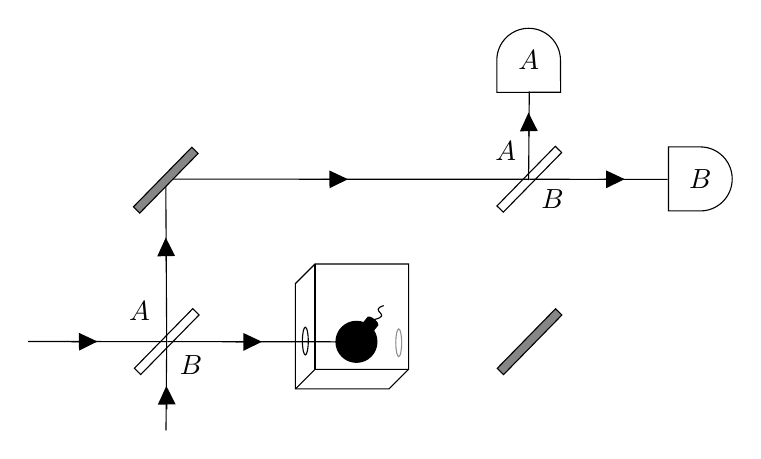
\begin{tikzpicture}[x=0.75pt,y=0.75pt,yscale=-1,xscale=1]
%uncomment if require: \path (0,300); %set diagram left start at 0, and has height of 300

%Shape: Rectangle [id:dp9015870766848293] 
\draw   (232.64,194.14) -- (260.76,165.42) -- (263.8,168.43) -- (235.68,197.15) -- cycle ;
%Straight Lines [id:da8378126329447328] 
\draw    (248.22,181.29) -- (247.88,224) ;


%Straight Lines [id:da4203005431788527] 
\draw    (181.51,181.2) -- (248.22,181.29) ;


%Straight Lines [id:da0243171970681888] 
\draw    (247.78,103.5) -- (248.22,181.29) ;


%Shape: Rectangle [id:dp6223611714942476] 
\draw   (407.34,115.91) -- (435.46,87.19) -- (438.5,90.2) -- (410.38,118.92) -- cycle ;
%Straight Lines [id:da6198680343533711] 
\draw    (248.58,181.29) -- (339.64,181.38) ;


%Straight Lines [id:da46097237064220464] 
\draw    (248.33,103.01) -- (422.78,103.05) ;


%Straight Lines [id:da9742962817963474] 
\draw    (422.92,103.05) -- (489.62,103.14) ;


%Straight Lines [id:da6938242067138403] 
\draw    (422.92,60.82) -- (422.59,103.53) ;


%Shape: Rectangle [id:dp9634903942334572] 
\draw  [color={rgb, 255:red, 0; green, 0; blue, 0 }  ,draw opacity=1 ][fill={rgb, 255:red, 134; green, 134; blue, 134 }  ,fill opacity=1 ] (232.19,116.35) -- (260.32,87.63) -- (263.36,90.64) -- (235.23,119.36) -- cycle ;
%Straight Lines [id:da5813104731210839] 
\draw    (202.27,181.35) -- (212.87,181.26) ;
\draw [shift={(214.87,181.24)}, rotate = 539.49] [fill={rgb, 255:red, 0; green, 0; blue, 0 }  ][line width=0.75]  [draw opacity=0] (8.93,-4.29) -- (0,0) -- (8.93,4.29) -- cycle    ;

%Straight Lines [id:da44635174735191185] 
\draw    (248.27,213.87) -- (248.09,204.64) ;
\draw [shift={(248.05,202.64)}, rotate = 448.87] [fill={rgb, 255:red, 0; green, 0; blue, 0 }  ][line width=0.75]  [draw opacity=0] (8.93,-4.29) -- (0,0) -- (8.93,4.29) -- cycle    ;

%Straight Lines [id:da0008306331435172787] 
\draw    (248,142.39) -- (247.82,133.17) ;
\draw [shift={(247.78,131.17)}, rotate = 448.87] [fill={rgb, 255:red, 0; green, 0; blue, 0 }  ][line width=0.75]  [draw opacity=0] (8.93,-4.29) -- (0,0) -- (8.93,4.29) -- cycle    ;

%Straight Lines [id:da07946196970039154] 
\draw    (322.96,103.14) -- (333.56,103.05) ;
\draw [shift={(335.56,103.03)}, rotate = 539.49] [fill={rgb, 255:red, 0; green, 0; blue, 0 }  ][line width=0.75]  [draw opacity=0] (8.93,-4.29) -- (0,0) -- (8.93,4.29) -- cycle    ;

%Straight Lines [id:da07206766467829073] 
\draw    (456.27,103.1) -- (466.87,103) ;
\draw [shift={(468.87,102.99)}, rotate = 539.49] [fill={rgb, 255:red, 0; green, 0; blue, 0 }  ][line width=0.75]  [draw opacity=0] (8.93,-4.29) -- (0,0) -- (8.93,4.29) -- cycle    ;

%Straight Lines [id:da618984745312871] 
\draw    (422.75,82.18) -- (422.57,72.95) ;
\draw [shift={(422.53,70.95)}, rotate = 448.87] [fill={rgb, 255:red, 0; green, 0; blue, 0 }  ][line width=0.75]  [draw opacity=0] (8.93,-4.29) -- (0,0) -- (8.93,4.29) -- cycle    ;

%Flowchart: Delay [id:dp8754933152186037] 
\draw   (490.01,87.47) -- (505.34,87.47) .. controls (513.81,87.47) and (520.68,94.38) .. (520.68,102.89) .. controls (520.68,111.41) and (513.81,118.31) .. (505.34,118.31) -- (490.01,118.31) -- cycle ;
%Flowchart: Delay [id:dp7631066454512347] 
\draw   (407.32,61.21) -- (407.27,45.79) .. controls (407.24,37.28) and (414.08,30.35) .. (422.55,30.32) .. controls (431.02,30.29) and (437.91,37.17) .. (437.94,45.69) -- (438,61.11) -- cycle ;
%Shape: Rectangle [id:dp0901747104841557] 
\draw  [color={rgb, 255:red, 0; green, 0; blue, 0 }  ,draw opacity=1 ][fill={rgb, 255:red, 134; green, 134; blue, 134 }  ,fill opacity=1 ] (407.45,194.18) -- (435.57,165.46) -- (438.61,168.47) -- (410.49,197.19) -- cycle ;
%Shape: Circle [id:dp21556459507248826] 
\draw  [fill={rgb, 255:red, 0; green, 0; blue, 0 }  ,fill opacity=1 ] (329.77,181.38) .. controls (329.77,175.92) and (334.19,171.5) .. (339.64,171.5) .. controls (345.1,171.5) and (349.52,175.92) .. (349.52,181.38) .. controls (349.52,186.83) and (345.1,191.25) .. (339.64,191.25) .. controls (334.19,191.25) and (329.77,186.83) .. (329.77,181.38) -- cycle ;
%Flowchart: Stored Data [id:dp7749919190363537] 
\draw  [fill={rgb, 255:red, 0; green, 0; blue, 0 }  ,fill opacity=1 ] (349.91,173.29) -- (346.81,177.19) .. controls (347.14,176.78) and (346.34,175.61) .. (345.04,174.57) .. controls (343.74,173.54) and (342.42,173.03) .. (342.09,173.44) -- (345.19,169.54) .. controls (345.51,169.13) and (346.84,169.64) .. (348.14,170.67) .. controls (349.44,171.71) and (350.24,172.88) .. (349.91,173.29) -- cycle ;
%Curve Lines [id:da27499232782476213] 
\draw    (348.14,170.67) .. controls (357.52,168.42) and (345.02,166.42) .. (352.77,163.92) ;


%Shape: Cube [id:dp8083755578351033] 
\draw   (364.78,194.63) -- (355.37,204.03) -- (310.25,204.03) -- (310.25,153.31) -- (319.66,143.9) -- (364.78,143.9) -- cycle ; \draw   (310.25,204.03) -- (319.66,194.63) -- (364.78,194.63) ; \draw   (319.66,194.63) -- (319.66,143.9) ;
%Shape: Ellipse [id:dp48925511756322826] 
\draw   (313.6,181) .. controls (313.6,177.32) and (314.23,174.33) .. (315.02,174.33) .. controls (315.8,174.33) and (316.43,177.32) .. (316.43,181) .. controls (316.43,184.68) and (315.8,187.67) .. (315.02,187.67) .. controls (314.23,187.67) and (313.6,184.68) .. (313.6,181) -- cycle ;
%Shape: Ellipse [id:dp9235217248592085] 
\draw  [color={rgb, 255:red, 0; green, 0; blue, 0 }  ,draw opacity=0.44 ][fill={rgb, 255:red, 0; green, 0; blue, 0 }  ,fill opacity=0 ] (358.6,181.83) .. controls (358.6,178.15) and (359.23,175.17) .. (360.02,175.17) .. controls (360.8,175.17) and (361.43,178.15) .. (361.43,181.83) .. controls (361.43,185.52) and (360.8,188.5) .. (360.02,188.5) .. controls (359.23,188.5) and (358.6,185.52) .. (358.6,181.83) -- cycle ;
%Straight Lines [id:da20174840319475407] 
\draw    (281.51,181.44) -- (292.11,181.35) ;
\draw [shift={(294.11,181.33)}, rotate = 539.49] [fill={rgb, 255:red, 0; green, 0; blue, 0 }  ][line width=0.75]  [draw opacity=0] (8.93,-4.29) -- (0,0) -- (8.93,4.29) -- cycle    ;


% Text Node
\draw (259.93,192.77) node   {$B$};
% Text Node
\draw (235.17,166.66) node   {$A$};
% Text Node
\draw (411.53,89.42) node   {$A$};
% Text Node
\draw (434.19,112.76) node   {$B$};
% Text Node
\draw (505.34,102.89) node   {$B$};
% Text Node
\draw (422.61,45.74) node   {$A$};


\end{tikzpicture}
\end{center}
\caption{Nel caso in cui vi sia effettivamente una bomba, solo uno dei due percorsi è possibile, e perciò non si ha alcuna interferenza nel secondo beam-splitter.\label{fig:interferometro-boom}}
\end{figure}
\end{itemize}

Notiamo che se la scatola è vuota, il rivelatore $A$ non trova mai il fotone. Perciò, se troviamo il fotone in $A$ sappiamo immediatamente che la bomba è presente. Ciò succede in un caso su $4$: abbiamo allora un modo per misurare la presenza  o meno di un oggetto \textbf{senza} interagire con esso in alcun modo.\\
Per quanto ciò sia paradossale, tale setup - il cosiddetto \textit{detector di bombe} di Elitzur-Vaidman - è stato realizzato sperimentalente (sostituendo la bomba con un ostacolo meno pericoloso).\\
Per di più si trova (\cite{detection-free}) che è possibile concatenare tanti circuiti simili per aumentare (arbitrariamente) la probabilità di rivelazione senza interazione.\\

\begin{expl}
\textbf{Interpretazione del tester Elitzur-Vaidman}. Un modo di pensare gli esiti dell'esperimento sta nel considerare la bomba come un \textit{sistema interagente}. Se è presente, allora interagisce con la funzione d'onda del fotone, e la fa collassare su uno dei due percorsi possibili. Se non è presente, invece, non avviene alcun collasso, e la funzione d'onda è libera di interferire con se stessa nel secondo BS. In un certo senso, perciò, l'apparato non sta facendo altro che determinare se una interazione sia avvenuta o meno. Interpretando tale interazione non unitaria come una \textit{misurazione}, pittorescamente si potrebbe affermare che il tester Elitzur-Vaidman \q{misura l'avvenire o meno di un'altra misura}.
\end{expl}

Possibilità del genere hanno applicazione, per esempio, per ridurre la quantità di radiazioni assorbite da un tessuto durante una radiografia, dato che parte dei fotoni utilizzati portano \textit{informazione utile} senza interazione con il paziente.

\section{Effetto Zenone quantistico}
\subsection{I paradossi di Zenone}
I \textbf{paradossi di Zenone} furono una serie di paradossi ideati nell'antica Grecia.\\
Il più conosciuto è quello di \textit{Achille e la tartaruga}, che percorre il seguente ragionamento:
\begin{enumerate}
\item Achille (detto \textit{pie' veloce} per la sua formidabile rapidita) viene sfidato da una tartaruga ad una gara di corsa. Per rendere un minimo più equa la competizione, alla tartaruga è concesso partire con una certa distanza di vantaggio.
\item Achille raggiunge la tartaruga in un certo tempo $t_1$, percorrendo la distanza $x$ a velocità $v_A$. Ma nel frattempo la tartaruga si è spostata di un ulteriore $x_2 = v_t t_1$.
\item Achille copre la distanza $x_2$ in un tempo $t_2$, ma nel frattempo la tartaruga si posta ancora di una distanza $x_3 = v_t t_2$, e così via. 
\end{enumerate}
Poiché la serie \textit{continua all'infinito}, si potrebbe pensare che Achille non possa mai raggiungere la tartaruga. Serviranno i concetti di analisi matematica, per cui una serie infinita può convergere a un valore finito, per risolvere il problema.\\

Un altro paradosso è quello della \textbf{freccia}, secondo cui un dardo non può mai raggiungere nessuna destinazione, poiché ad ogni istante di tempo è \textit{fermo}, e la somma di \textit{infiniti istanti stazionaria} non può - almeno in principio - costituire un moto.\\

L'esperienza comune dimostra come il moto avvenga in realtà senza alcun problema. Il vero paradosso sorge allora quando, in \MQ, si scopre che il \textit{paradosso della freccia} è davvero possibile: misurando \textit{tante} volte una particella è possibile \textit{arrestare} la sua evoluzione temporale!
\end{document}

